\section{Comments}

\begin{itemize}
	\item The deterministic approximation of the reconstruction term feels very heurstic-ish. Is there a better method to generalize this to a large set of non-linearities?
	\item Having a selective hyper-parameter throughout the network is an interesting idea. Was the inverse gamma the only prior considered?
	\item Appendix is extensive and a good reference.
\end{itemize}

% \newpage
% \begin{figure}[t]
% \centering
% 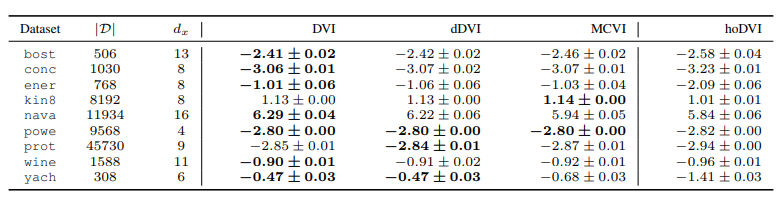
\includegraphics[scale=.45]{fig/results.png}
% \caption{Average log-likelihood on UCI datasets.}
% \end{figure}